\documentclass[a4paper,12pt]{article}

% --- PAQUETES ESENCIALES ---
\usepackage[utf8]{inputenc}
\usepackage[T1]{fontenc}
\usepackage[english]{babel}
\usepackage{geometry}
\usepackage{graphicx}
\graphicspath{{figures/}}
\usepackage{tikz}
\usetikzlibrary{shapes.geometric, arrows.meta, positioning}
\usepackage{xcolor}
\usepackage{tcolorbox}
\usepackage{longtable}
\usepackage{booktabs}
\usepackage{fancyhdr}
\usepackage{hyperref}
\usepackage{amsmath, amssymb}
\usepackage{enumitem}
\usepackage{calc}
\usepackage{csquotes}
\usepackage{setspace}
\usepackage{xfp}  % for math calculation

% =====================================================
% Variables auto-generated by 04_augmentation_training.py
% Includes rigorous bootstrap CIs and non-parametric p-values
% =====================================================

% --- Experiment A: Baseline Stacking (No Feat Sel, No Aug) ---
\newcommand{\ExpARTwoMean}{0.8072}
\newcommand{\ExpAMae}{0.4881}
\newcommand{\ExpARTwoCILow}{0.7275}
\newcommand{\ExpARTwoCIHigh}{0.8624}

% --- Experiment B: Permutation Importance Selection ---
\newcommand{\ExpBRTwoMean}{0.8082}
\newcommand{\ExpBMae}{0.4876}
\newcommand{\ExpBRTwoCILow}{0.7296}
\newcommand{\ExpBRTwoCIHigh}{0.8634}
\newcommand{\ExpBNFeaturesTotal}{2048}
\newcommand{\ExpBNFeaturesSelected}{1754}

% --- Experiment C: Feature Selection + Gaussian Augmentation ---
\newcommand{\ExpCRTwoMean}{0.7796}
\newcommand{\ExpCMae}{0.5332}
\newcommand{\ExpCRTwoCILow}{0.6860}
\newcommand{\ExpCRTwoCIHigh}{0.8451}
\newcommand{\ExpCAugFactor}{3}
\newcommand{\ExpCAugSizeTrain}{1926}
\newcommand{\ExpCNoiseLevels}{0.01, 0.001}

% --- Reference Benchmarks ---
\newcommand{\PaperBaselineRTwo}{0.75}
\newcommand{\PaperSelectedRTwo}{0.82}
\newcommand{\PaperFinalRTwo}{0.85}

% --- Rigorous Statistical Evaluations vs Benchmarks ---
\newcommand{\ExpAVsPaperBaselineInCI}{true}
\newcommand{\ExpAVsPaperBaselinePBoot}{0.1420}
\newcommand{\ExpAVsPaperBaselineSig}{false}
\newcommand{\ExpAVsPaperSelectedInCI}{true}
\newcommand{\ExpAVsPaperSelectedPBoot}{0.6850}
\newcommand{\ExpAVsPaperSelectedSig}{false}
\newcommand{\ExpAVsPaperFinalInCI}{true}
\newcommand{\ExpAVsPaperFinalPBoot}{0.1520}
\newcommand{\ExpAVsPaperFinalSig}{false}
\newcommand{\ExpBVsPaperBaselineInCI}{true}
\newcommand{\ExpBVsPaperBaselinePBoot}{0.1350}
\newcommand{\ExpBVsPaperBaselineSig}{false}
\newcommand{\ExpBVsPaperSelectedInCI}{true}
\newcommand{\ExpBVsPaperSelectedPBoot}{0.7020}
\newcommand{\ExpBVsPaperSelectedSig}{false}
\newcommand{\ExpBVsPaperFinalInCI}{true}
\newcommand{\ExpBVsPaperFinalPBoot}{0.1580}
\newcommand{\ExpBVsPaperFinalSig}{false}
\newcommand{\ExpCVsPaperBaselineInCI}{true}
\newcommand{\ExpCVsPaperBaselinePBoot}{0.5390}
\newcommand{\ExpCVsPaperBaselineSig}{false}
\newcommand{\ExpCVsPaperSelectedInCI}{true}
\newcommand{\ExpCVsPaperSelectedPBoot}{0.2590}
\newcommand{\ExpCVsPaperSelectedSig}{false}
\newcommand{\ExpCVsPaperFinalInCI}{false}
\newcommand{\ExpCVsPaperFinalPBoot}{0.0330}
\newcommand{\ExpCVsPaperFinalSig}{true}

% Auto-generated by 3DOCKING.py
% Include with: % Auto-generated by 3DOCKING.py
% Include with: % Auto-generated by 3DOCKING.py
% Include with: \input{docking_variables.tex}

\newcommand{\DockNTotal}{10}
\newcommand{\DockNValidated}{0}
\newcommand{\DockNDiscordant}{4}
\newcommand{\DockExhaustiveness}{32}
\newcommand{\DockBoxSize}{20.0}
\newcommand{\DockCenterX}{17.394}
\newcommand{\DockCenterY}{68.757}
\newcommand{\DockCenterZ}{-68.051}
\newcommand{\DockPearsonR}{-0.662}
\newcommand{\DockPearsonP}{0.0371}
\newcommand{\DockBestCandidate}{FolicAcid}
\newcommand{\DockBestMLpIC50}{8.1913}
\newcommand{\DockBestDockScore}{-5.55}


\newcommand{\DockNTotal}{10}
\newcommand{\DockNValidated}{0}
\newcommand{\DockNDiscordant}{4}
\newcommand{\DockExhaustiveness}{32}
\newcommand{\DockBoxSize}{20.0}
\newcommand{\DockCenterX}{17.394}
\newcommand{\DockCenterY}{68.757}
\newcommand{\DockCenterZ}{-68.051}
\newcommand{\DockPearsonR}{-0.662}
\newcommand{\DockPearsonP}{0.0371}
\newcommand{\DockBestCandidate}{FolicAcid}
\newcommand{\DockBestMLpIC50}{8.1913}
\newcommand{\DockBestDockScore}{-5.55}


\newcommand{\DockNTotal}{10}
\newcommand{\DockNValidated}{4}
\newcommand{\DockNDiscordant}{0}
\newcommand{\DockExhaustiveness}{32}
\newcommand{\DockBoxSize}{20.0}
\newcommand{\DockCenterX}{3.689}
\newcommand{\DockCenterY}{39.992}
\newcommand{\DockCenterZ}{-62.818}
\newcommand{\DockSpearmanRho}{-0.394}
\newcommand{\DockSpearmanP}{0.2600}
\newcommand{\DockBestCandidate}{Pralatrexate}
\newcommand{\DockBestMLpIC}{7.6354}
\newcommand{\DockBestDockScore}{-9.43}
\newcommand{\ChlorambucilMLpIC}{6.37}
\newcommand{\ChlorambucilDockScore}{-6.21}

\newcommand{\ChemPropDMPNNFoldRTwoMean}{0.6906}
\newcommand{\ChemPropDMPNNFoldMae}{0.5267}
\newcommand{\ChemPropDMPNNFoldRTwoStd}{0.0547}
\newcommand{\ChemPropDMPNNFoldCILow}{0.6692}
\newcommand{\ChemPropDMPNNFoldCIHigh}{0.7120}

% =====================================================
% Nested CV Benchmark Variables (Auto-generated)
% =====================================================

\newcommand{\NCompounds}{756}
\newcommand{\OuterKFolds}{5}
\newcommand{\OuterRepeats}{5}
\newcommand{\TotalOuterFolds}{25}
\newcommand{\InnerKFolds}{5}
\newcommand{\MaxComboSize}{3}

\newcommand{\PaperBaselineRTwo}{0.75}
\newcommand{\PaperSelectedRTwo}{0.82}
\newcommand{\PaperFinalRTwo}{0.85}

\newcommand{\MorganRTwoMean}{0.7417}
\newcommand{\MorganRTwoStd}{0.0493}
\newcommand{\MorganNFolds}{25}
\newcommand{\MorganBestArchitecture}{LGBM+XGB+SVM}
\newcommand{\MorganBestArchitectureSafe}{LGBMXGBSVM}
\newcommand{\MorganStability}{12.0}
\newcommand{\MorganMaeMean}{0.4841}
\newcommand{\MorganNFeaturesTotal}{2048}
\newcommand{\MorganNFeaturesSelectedMean}{2048.0}
\newcommand{\RdkitTwoDThreeDFpRTwoMean}{0.7348}
\newcommand{\RdkitTwoDThreeDFpRTwoStd}{0.0614}
\newcommand{\RdkitTwoDThreeDFpNFolds}{25}
\newcommand{\RdkitTwoDThreeDFpBestArchitecture}{ET+LGBM+SVM}
\newcommand{\RdkitTwoDThreeDFpBestArchitectureSafe}{ETLGBMSVM}
\newcommand{\RdkitTwoDThreeDFpStability}{32.0}
\newcommand{\RdkitTwoDThreeDFpMaeMean}{0.4835}
\newcommand{\RdkitTwoDThreeDFpNFeaturesTotal}{2275}
\newcommand{\RdkitTwoDThreeDFpNFeaturesSelectedMean}{1262.8}
\newcommand{\RdkitTwoDFpRTwoMean}{0.7297}
\newcommand{\RdkitTwoDFpRTwoStd}{0.0592}
\newcommand{\RdkitTwoDFpNFolds}{25}
\newcommand{\RdkitTwoDFpBestArchitecture}{ET+LGBM+SVM}
\newcommand{\RdkitTwoDFpBestArchitectureSafe}{ETLGBMSVM}
\newcommand{\RdkitTwoDFpStability}{20.0}
\newcommand{\RdkitTwoDFpMaeMean}{0.4885}
\newcommand{\RdkitTwoDFpNFeaturesTotal}{2265}
\newcommand{\RdkitTwoDFpNFeaturesSelectedMean}{1261.8}
\newcommand{\RdkitTwoDRTwoMean}{0.6785}
\newcommand{\RdkitTwoDRTwoStd}{0.0639}
\newcommand{\RdkitTwoDNFolds}{25}
\newcommand{\RdkitTwoDBestArchitecture}{ET+LGBM+SVM}
\newcommand{\RdkitTwoDBestArchitectureSafe}{ETLGBMSVM}
\newcommand{\RdkitTwoDStability}{32.0}
\newcommand{\RdkitTwoDMaeMean}{0.5301}
\newcommand{\RdkitTwoDNFeaturesTotal}{217}
\newcommand{\RdkitTwoDNFeaturesSelectedMean}{181.4}

\newcommand{\PValueMorganVsPaperBaseline}{0.7558}
\newcommand{\TStatMorganVsPaperBaseline}{-0.315}
\newcommand{\SigDiffMorganVsPaperBaseline}{false}
\newcommand{\PValueMorganVsPaperSelected}{0.0069}
\newcommand{\TStatMorganVsPaperSelected}{-2.953}
\newcommand{\SigDiffMorganVsPaperSelected}{true}
\newcommand{\PValueMorganVsPaperFinal}{0.0004}
\newcommand{\TStatMorganVsPaperFinal}{-4.084}
\newcommand{\SigDiffMorganVsPaperFinal}{true}
\newcommand{\PValueRdkitTwoDThreeDFpVsPaperBaseline}{0.6492}
\newcommand{\TStatRdkitTwoDThreeDFpVsPaperBaseline}{-0.461}
\newcommand{\SigDiffRdkitTwoDThreeDFpVsPaperBaseline}{false}
\newcommand{\PValueRdkitTwoDThreeDFpVsPaperSelected}{0.0165}
\newcommand{\TStatRdkitTwoDThreeDFpVsPaperSelected}{-2.578}
\newcommand{\SigDiffRdkitTwoDThreeDFpVsPaperSelected}{true}
\newcommand{\PValueRdkitTwoDThreeDFpVsPaperFinal}{0.0019}
\newcommand{\TStatRdkitTwoDThreeDFpVsPaperFinal}{-3.485}
\newcommand{\SigDiffRdkitTwoDThreeDFpVsPaperFinal}{true}
\newcommand{\PValueRdkitTwoDVsPaperBaseline}{0.0486}
\newcommand{\TStatRdkitTwoDVsPaperBaseline}{-2.077}
\newcommand{\SigDiffRdkitTwoDVsPaperBaseline}{true}
\newcommand{\PValueRdkitTwoDVsPaperSelected}{0.0004}
\newcommand{\TStatRdkitTwoDVsPaperSelected}{-4.111}
\newcommand{\SigDiffRdkitTwoDVsPaperSelected}{true}
\newcommand{\PValueRdkitTwoDVsPaperFinal}{0.0000}
\newcommand{\TStatRdkitTwoDVsPaperFinal}{-4.982}
\newcommand{\SigDiffRdkitTwoDVsPaperFinal}{true}
\newcommand{\PValueRdkitTwoDFpVsPaperBaseline}{0.5309}
\newcommand{\TStatRdkitTwoDFpVsPaperBaseline}{-0.636}
\newcommand{\SigDiffRdkitTwoDFpVsPaperBaseline}{false}
\newcommand{\PValueRdkitTwoDFpVsPaperSelected}{0.0092}
\newcommand{\TStatRdkitTwoDFpVsPaperSelected}{-2.833}
\newcommand{\SigDiffRdkitTwoDFpVsPaperSelected}{true}
\newcommand{\PValueRdkitTwoDFpVsPaperFinal}{0.0009}
\newcommand{\TStatRdkitTwoDFpVsPaperFinal}{-3.774}
\newcommand{\SigDiffRdkitTwoDFpVsPaperFinal}{true}

\newcommand{\TopModeOne}{Morgan}
\newcommand{\TopModeTwo}{RdkitTwoDThreeDFp}
\newcommand{\PairedTTestStat}{0.464}
\newcommand{\PairedTTestP}{0.6471}

\newcommand{\WinnerMode}{Morgan}
\newcommand{\WinnerRTwoMean}{0.7417}
\newcommand{\WinnerRTwoStd}{0.0493}

% Auto-generated by 06_redocking_validation.py pipeline
\newcommand{\RedockRMSD}{0.32}
\newcommand{\RedockEnergy}{-7.91}
\newcommand{\RedockThreshold}{2.0}
\newcommand{\RedockLigand}{CP6}
\newcommand{\RedockChain}{B}
\newcommand{\RedockCenterX}{3.689}
\newcommand{\RedockCenterY}{39.992}
\newcommand{\RedockCenterZ}{-62.818}
\newcommand{\RedockCenterOffset}{0.001}
\newcommand{\RedockValidated}{true}

% --- CONFIGURACIÓN DE MÁRGENES ---
\geometry{
	a4paper,
	left=2.5cm,
	right=2.5cm, 
	top=2cm,
	bottom=3.5cm,
	headsep=0.8cm,
	footskip=1cm
}

% --- HEADHEIGHT PARA FANCYHDR ---
\setlength{\headheight}{55pt}

% --- COLORES PERSONALIZADOS ---
\definecolor{utemBlue}{RGB}{0, 51, 102}
\definecolor{utemLight}{RGB}{230, 240, 255}
\definecolor{accentColor}{RGB}{200, 50, 50}

% --- DATOS EDITABLES ---
\newcommand{\NombreAlumno}{Andrey Vinajera Zamora}
\newcommand{\RUT}{99900286-2}
\newcommand{\Asignatura}{\textbf{Redacción Científica}}
\newcommand{\Profesor}{Dr. Tomás Veloz}
\newcommand{\TituloTarea}{Tarea 2.1 }
\newcommand{\FechaEntrega}{\today}

% --- ESTILO DE CAJAS ---
\tcbuselibrary{skins, breakable}

\newtcolorbox{pregunta}[1]{
	colback=white,
	colframe=utemBlue,
	fonttitle=\bfseries,
	title={#1},
	breakable,
	arc=4pt,
	before skip=6pt,
	after skip=6pt
}

% --- HEADER Y FOOTER ---
\pagestyle{fancy}
\fancyhf{}
\fancyhead[L]{
\includegraphics[height=1.2cm]{assets/logos/UTEM.jpeg}}
\fancyhead[R]{\small\textbf{\Asignatura}  \\ \footnotesize \NombreAlumno}
\fancyfoot[C]{\thepage}
\renewcommand{\headrulewidth}{0.4pt}
\renewcommand{\headrule}{\hbox to\headwidth{\color{utemBlue}\leaders\hrule height \headrulewidth\hfill}}

% --- HYPERREF CONFIG ---
\hypersetup{
	colorlinks=true,
	linkcolor=utemBlue,
	urlcolor=accentColor,
	citecolor=utemBlue,
	pdfstartview=FitH
}

% --- COMANDO PARA ESPACIO DE RESPUESTA ---
\newcommand{\espacioRespuesta}[1][8]{
	\vspace{#1\baselineskip}
	\noindent\rule{\linewidth}{0.4pt}
}

\begin{document}
	
	% --- PORTADA ---
	
	

	
	%\newpage
	\setcounter{page}{1}
	

\begin{center}
	\begin{singlespace}
		 \textbf{PAPER} \\
		\vspace{0.5cm}
		 \textbf{When simple wins: leakage-free benchmarking of classical Machine learning vs. graph neural networks in low-data bioactivity prediction}
	\end{singlespace}
	
\end{center}

\begin{abstract}

\end{abstract}

\textbf{Keywords:} 
	Quantitative Structure-Activity Relationship, Low-Data Regimes, Nested Cross-Validation, Data Leakage, Graph Neural Networks, Molecular Docking

\section{Introduction}

% ==========================================
% 1. SECTION 1.1
% ==========================================

\subsection{Predictive Modeling in Low-Data Bioactivity Regimes}

Predictive modeling in quantitative structure-activity relationships (QSAR) operates under strict constraints when data is scarce \cite{winkler2026}. Under these conditions, simpler interpretable approaches—such as multivariate linear regression or classical tree-based ensembles—frequently match or exceed the prediction reliability of complex artificial neural networks \cite{hadas2023, xiewt2023}. These parsimonious models maintain higher bias and lower variance. They resist the extreme sensitivity to random fluctuations that plagues overparameterized algorithms, particularly when supplied with robust, quantum-chemically derived descriptors \cite{xiewt2023}.

Small datasets inherently invite overfitting. This bottleneck worsens exponentially when the dimensionality of molecular descriptors exceeds the available sample size \cite{hawkins2004, godarzi2013}. To circumvent data sparsity, contemporary workflows frequently deploy data augmentation (DAU) or synthetic sample generation to artificially expand the training manifold \cite{gerz2026, tyler2025}. However, these interventions demand substantial computational overhead \cite{tyler2025, calle2025}. More critically, improper DAU application obscures the true predictive capacity of the base algorithms. When augmentation precedes dataset partitioning (the ``augment-then-split'' fallacy), it violates independent and identically distributed (i.i.d.) assumptions. Models memorize synthetic artifacts and latent data dependencies rather than learning genuine physicochemical rules, yielding artificially inflated performance metrics \cite{gerz2026, john2025, kannoth2024}.

Evaluating complex architectures in these regimes requires absolute methodological isolation. Hyperparameter tuning on small samples with large parameter spaces inevitably leads to model selection bias \cite{cawley2010}. Consequently, assessing machine learning architectures in isolation provides zero evidence of real-world utility unless the model selection procedure itself undergoes rigorous validation. Double (or nested) cross-validation becomes mandatory to decouple model building from performance estimation \cite{bauman2014, cawley2010}. Standard k-fold cross-validation systematically overestimates explorative capabilities \cite{kyrali2022, xiong2020}, and generative deep learning struggles to extrapolate within sparse, discrete chemical spaces like Simplified Molecular-Input Line-Entry System (SMILES) strings \cite{yifan2023}. To preserve methodological integrity, any generative or augmentative process must remain strictly confined to the training folds after establishing an independent partition \cite{gerz2026, john2025}.

To safely harness overparameterized models \cite{winkler2026} without succumbing to the overfitting trap, empirical safeguards against chance correlation are non-negotiable. Techniques such as y-randomization (response shuffling) explicitly verify that the algorithm maps true chemical relationships rather than memorizing random noise \cite{rucker2007}. Although frequently recommended in literature, its empirical execution is routinely omitted in modern deep learning QSAR studies; enforcing this protocol is therefore essential to definitively rule out chance correlation before advancing candidates to virtual screening. When descriptors undergo meticulous curation and pass these randomization checks, machine learning effectively guides rational design—successfully discriminating potent bioactives, such as Amyloid-$\beta$ aggregation inhibitors, from decoys \cite{avantika2025}. 

Alternatively, transfer learning bypasses data scarcity by adapting base networks optimized on massive source domains \cite{samuel2023}. By enforcing reduced learning rates during fine-tuning \cite{damilola2025} and prioritizing efficient convolutional architectures over heavier Transformer models \cite{riza2025}, researchers can navigate class imbalance and model selection bias in low-resource settings.

% ==========================================
% 1. SECTION 1.2
% ==========================================
\subsection{Domain-Engineered Features versus End-to-End Representation Learning}

Traditional feature-based machine learning relies on domain-engineered descriptors and molecular fingerprints \cite{rajesh2026}. Representations such as Morgan (ECFP4) encode structural topologies, while physicochemical and 3D descriptors capture specific molecular interactions deterministically without requiring massive training corpora \cite{avantika2025, beatrice2026, xiewt2023}. Embedding theoretical chemistry directly into the model ensures high interpretability and algorithmic transparency \cite{xiewt2023}. However, accumulating these handcrafted features generates highly dimensional, redundant matrices \cite{godarzi2013, hadas2023}. In restricted datasets, this redundancy amplifies computational costs and exacerbates the feature selection bottleneck \cite{godarzi2013, hadas2023}.

End-to-end representation learning bypasses manual feature selection. Deep learning paradigms—including Autoencoders (VAEs), Generative Adversarial Networks (GANs), and Graph Neural Networks (GNNs)—autonomously map discrete molecular topologies into continuous latent spaces to model complex, nonlinear interactions \cite{abul2026, rajesh2026, yifan2023}. Similarly, Chemical Language Processing (CLP) applies natural language techniques to string representations like SMILES \cite{riza2025}. Yet, learning representations in discrete chemical spaces remains intrinsically fragile. Altering a single character in a SMILES string can irreparably invalidate the entire molecular structure \cite{yifan2023}.

The utility of deep learning complexity in low-data regimes remains highly contested. These algorithms require dense data manifolds, rendering representation learning ineffective when ground-truth labels are scarce \cite{sotirios2025}. To circumvent this limitation in \textit{Toxoplasma gondii} dihydrofolate reductase (TgDHFR) inhibition, recent studies deploy highly complex pipelines. \cite{karimova2025} employed Gaussian noise-based data augmentation and deep neural network (DNN) ensembles to stabilize training on a restricted dataset, elevating their baseline $R^2$ from \PaperBaselineRTwo{} to \PaperFinalRTwo{}. This intervention prompts a critical evaluation: is synthetic data generation strictly necessary to achieve predictive reliability? Parsimonious classical ensembles frequently match or exceed the predictive fidelity of deep architectures in data-scarce scenarios, avoiding the catastrophic overfitting inherent to unregularized overparameterization \cite{beatrice2026, hadas2023, rajesh2026, salman2023, samuel2023, xiewt2023}.

Traditional skepticism toward nonlinear models in limited-data scenarios is evolving \cite{Dalmau2025}. Properly regularized nonlinear algorithms, hybridized with structured linear priors, achieve competitive results comparable to robust classical methods \cite{Dalmau2025, salman2023}. Transfer learning serves as a primary catalyst for this shift. Fine-tuning pretrained networks like ChemBERTa allows researchers to extract accurate representation learning predictions using only dozens of target data points \cite{latefa2025, samuel2023}.

% ==========================================
% 1. SECTION 1.3
% ==========================================
\subsection{Methodological Rigor and the Threat of Data Leakage in Molecular Modeling}

Data leakage—the unintended introduction of test data information into the training process—is a statistically silent error that fundamentally undermines the validity of machine learning evaluations by inflating metrics without triggering code warnings \cite{brva2026, gerz2026}. In low-data QSAR modeling, this vulnerability frequently manifests across two primary vectors: preprocessing and model selection. When transformations like feature scaling, imputation, or variance-based filtering are applied globally across an entire dataset, the algorithm gains illicit knowledge of the test distribution. This violation of the independent and identically distributed (i.i.d.) assumption yields spuriously high performance estimates \cite{correa2025, lewis2023}.

Similarly, traditional internal validation often suffers from model selection bias. If a validation set continuously influences hyperparameter tuning, it loses its statistical independence. Highly parameterized architectures, such as deep neural networks, are particularly prone to exploiting this overlap. They adapt to noise and produce deceptively optimistic metrics that severely underestimate true generalization errors \cite{bauman2014, sotirios2025}. To preserve methodological integrity, model selection and preprocessing must operate as strictly encapsulated components of the fitting process. Insufficient reporting of these partitioning mechanics often confounds scientific literature, leading researchers to incorrectly attribute high performance to novel complex architectures when the success actually stems from silent data leakage \cite{rojas2026}.

% ==========================================
% 1. SECTION 1.4
% ==========================================

\subsection{Objectives and Principal Contributions}

This study bridges the gap between stringent statistical validation and advanced representation learning to accelerate targeted drug discovery in low-data regimes. Our principal contributions are defined as follows:

\begin{itemize}
	\item \textbf{Methodological Reproducibility and Leak-Free Validation:} Implementation of a fully transparent, reproducible Python pipeline built upon a rigorous $\OuterKFolds \times \OuterRepeats$ repeated nested cross-validation protocol (\TotalOuterFolds{} outer evaluations). This architecture ensures absolute statistical independence between hyperparameter optimization and model evaluation, eradicating model selection bias and data leakage.
	
	\item \textbf{Rigorous Statistical Inference in QSAR:} Introduction of the Nadeau-Bengio variance correction to molecular machine learning evaluations. By explicitly accounting for training set overlap across repeated folds, this framework resolves the pervasive issue of pseudoreplication in standard cross-validation. This methodological contribution enables mathematically sound hypothesis testing between architectures, preventing the Type I error inflation that frequently confounds model selection in cheminformatics.
	
	\item \textbf{Architectural Benchmarking in Data-Limited Regimes:} A comprehensive empirical comparison evaluating the predictive reliability of traditional domain-engineered classical ensembles against state-of-the-art Graph Neural Networks (specifically, the ChemProp Directed Message Passing Neural Network, D-MPNN) using a standardized reference dataset.
	
	\item \textbf{Empirical Validation of Parsimony over Complexity:} Explicit demonstration that simple classical machine learning ensembles achieve statistical parity ($R^2 \approx \PaperBaselineRTwo$) with baseline deep learning models reported in recent literature. This establishes that competitive predictive reliability can be attained "out-of-the-box," effectively eliminating the necessity for synthetic data augmentation and computationally expensive 3D geometric preprocessing in low-data regimes.
	
	\item \textbf{Translational Drug Repurposing Pipeline:} The integration of machine learning predictions with structure-based molecular docking. This hybrid pipeline systematically screens, identifies, and prioritizes FDA-approved compounds, providing a validated computational pathway for rapid therapeutic repurposing.
\end{itemize}
\section{Materials and Methods}
\newcommand{\boxheight}{3.85cm}
\begin{figure}[!h]
	\centering
	\resizebox{\textwidth}{!}{%
		\begin{tikzpicture}[
			font=\sffamily\scriptsize,
			>=Stealth,
			node distance=0.45cm,
			basebox/.style={
				thick,
				rounded corners=4pt,
				inner sep=6pt,
				anchor=center,
				align=center
			},
			phase1/.style={basebox, draw=blue!75!black, fill=blue!4},
			phase2/.style={basebox, draw=violet!75!black, fill=violet!4},
			phase3/.style={basebox, draw=teal!80!black, fill=teal!4},
			phase4/.style={basebox, draw=orange!85!black, fill=orange!4},
			phase5/.style={basebox, draw=green!60!black, fill=green!5},
			arrowline/.style={->, ultra thick, draw=gray!65}
			]
			
			% FASE 1: ML BENCHMARKING (5x5 Repeated NCV)
			\node[phase1] (box1) {
				\begin{minipage}[t][\boxheight][t]{3.15cm}
					\centering
					\textbf{\footnotesize Phase 1: ML Modeling} \par\vspace{2pt}\hrule\vspace{7pt}
					\textbf{Training Set:} \\$N = \NCompounds$ TgDHFR \par\vspace{4pt}
					\textbf{Validation:} \\$5 \times 5$ Repeated NCV \par\vspace{4pt}
					\textbf{Descriptors:} \\ECFP4, 2D, 2D/3D \par\vspace{4pt}
					\textbf{Ensemble:} \\Stacking + RidgeCV \par\vspace{4pt}
					\textbf{Ablation:} \\PI + Gaussian Noise
				\end{minipage}
			};
			
			% FASE 2: FDA SCREENING
			\node[phase2, right=of box1] (box2) {
				\begin{minipage}[t][\boxheight][t]{3.15cm}
					\centering
					\textbf{\footnotesize Phase 2: Virtual Screen} \par\vspace{2pt}\hrule\vspace{7pt}
					\textbf{Target Space:} \\FDA Approved \par\vspace{4pt}
					\textbf{Library Size:} \\$N \approx 1,700$ \par\vspace{4pt}
					\textbf{PhysChem:} MW \\$\le 1000$\,Da \par\vspace{4pt}
					\textbf{Applicability:} \\Isolation Forest \par\vspace{4pt}
					\textbf{Prioritized Set:} \\$N = 19$ candidates
				\end{minipage}
			};
			
			% FASE 3: MOLECULAR DOCKING
			\node[phase3, right=of box2] (box3) {
				\begin{minipage}[t][\boxheight][t]{3.15cm}
					\centering
					\textbf{\footnotesize Phase 3: 3D Consensus} \par\vspace{2pt}\hrule\vspace{7pt}
					\textbf{Receptor:} \\TgDHFR (6AOG, Ch.~\RedockChain{}) \par\vspace{4pt}
					\textbf{Engine:} \\AutoDock Vina \par\vspace{4pt}
					\textbf{Exhaustiveness:}\\ \DockExhaustiveness{} \par\vspace{4pt}
					\textbf{Redock Fidelity:} \\RMSD = \RedockRMSD{}\,\AA \par\vspace{4pt}
					\textbf{Consensus:} \\ML--Physics overlap
				\end{minipage}
			};
			
			% FASE 4: ADMET PROFILING
			\node[phase4, right=of box3] (box4) {
				\begin{minipage}[t][\boxheight][t]{3.15cm}
					\centering
					\textbf{\footnotesize Phase 4: ADMET Profiling} \par\vspace{2pt}\hrule\vspace{7pt}
					\textbf{Input:} \\Docking consensus set \par\vspace{4pt}
					\textbf{Druggability:} \\Lipinski Rule of 5 \par\vspace{4pt}
					\textbf{Route Profiling:} \\Caco-2 (Oral vs. IV) \par\vspace{4pt}
					\textbf{Safety Filter:} \\hERG ($P_\mathrm{block} < 0.5$) \par\vspace{4pt}
					\textbf{Framework:} \\TDC Benchmarks
				\end{minipage}
			};
			
			% OUTCOME / FINAL CANDIDATES
			\node[phase5, right=of box4] (box5) {
				\begin{minipage}[t][\boxheight][t]{3.15cm}
					\centering
					\textbf{\footnotesize Validated Candidates} \par\vspace{2pt}\hrule\vspace{5pt}
					\textbf{Pralatrexate} \par\vspace{1pt}
					\textit{Top Consensus Lead} \par
					$p\mathrm{IC}_{50} = \DockBestMLpIC$ \\$\DockBestDockScore$\,kcal/mol \par\vspace{4pt}
					\textbf{Pyrimethamine} \par\vspace{1pt}
					\textit{High-Efficiency Lead} \par
					$p\mathrm{IC}_{50} = 6.42$ \\$-7.34$\,kcal/mol \par\vspace{4pt}
					\hrule\vspace{3pt}
					\textit{\DockNValidated{} Hits Structurally Verified}
				\end{minipage}
			};
			
			% FLECHAS DE CONEXIÓN
			\draw[arrowline] (box1) -- (box2);
			\draw[arrowline] (box2) -- (box3);
			\draw[arrowline] (box3) -- (box4);
			\draw[arrowline] (box4) -- (box5);
			
		\end{tikzpicture}%
	}
	\caption{\textbf{Schematic overview of the multi-tier computational repurposing and validation pipeline.} 
		The hierarchical funnel integrates: (1) 2D ligand-based representation benchmarking under nested cross-validation, (2) applicability domain-constrained screening of FDA-approved compounds, (3) orthogonal physics-based consensus validation via molecular docking (AutoDock Vina), and (4) in silico ADMET profiling (Caco-2 permeability route categorization and hERG cardiotoxicity filtering) to isolate clinically viable TgDHFR candidates.}
	\label{fig:pipeline_flowchart}
	\vspace{-10pt}
\end{figure}

An overview of the multi-tier virtual screening pipeline implemented in this study is illustrated in Figure~\ref{fig:pipeline_flowchart}.

% ==========================================
% 2. SECTION 2.1
% ==========================================

\subsection{Bioactivity Benchmark Dataset and Curation}

This study utilizes a previously published benchmark of \textit{Toxoplasma gondii} dihydrofolate reductase (TgDHFR) enzyme inhibitors \cite{karimova2025}. By adopting the exact baseline dataset compiled by Karimova and Senanayake, we establish a strict methodological control. This framework isolates the predictive capacity of classical machine learning algorithms from computationally heavy statistical interventions. Deliberately omitting synthetic data augmentation during the primary benchmarking phase ensures that performance metrics reflect empirical ground-truth data rather than algorithmic artifacts.

Initial records merged drug-protein interaction parameters and SMILES structures from BindingDB with bioactivity data from ChEMBL \cite{karimova2025}. Automated standardization protocols, including salt stripping and structural validation, ensured chemical integrity \cite{damilola2025}. To mitigate experimental noise and prevent overfitting \cite{cherkasov2014, iwuala2025}, 117 compounds were systematically excluded from the initial 873 entries. This exclusion targeted organometallic complexes---which preclude 3D force-field generation---and molecules with undefined stereocenters that introduce severe conformational ambiguity.

For compounds exhibiting multiple $IC_{50}$ measurements across varying experimental conditions, we applied the Interquartile Range (IQR) method. Duplicate assays with a bioactivity variance exceeding 1.5 log units were discarded as statistical outliers \cite{karimova2025}. The remaining consistent entries were averaged to yield a single representative measurement per ligand. 

This curation protocol yielded a final benchmark of $N = 756$ unique small molecules. The continuous target variable was transformed into $pIC_{50}$ ($-\log_{10}(IC_{50})$) \cite{karimova2025}. This logarithmic conversion standardizes response values and compresses the active range, optimizing the target distribution for robust regression modeling.

To explicitly quantify the performance impact of synthetic data generation reported in the original literature, we implemented an isolated data augmentation protocol exclusively for post-benchmark ablation studies. Following a strict 15\% hold-out partition to prevent data leakage, training features underwent perturbation via additive Gaussian noise. Applying two distinct noise levels ($\sigma = 0.01$ and $\sigma = 0.001$) generated two synthetic variants per original molecule. This procedure effectively triplicated the training space while maintaining absolute isolation of the empirical test set.

% ==========================================
% 2. SECTION 2.2
% ==========================================

\subsection{Representation Spaces: Molecular Fingerprints and Conformational Descriptors}

To systematically evaluate the structure-activity relationship, the open-source cheminformatics library RDKit \cite{landrum2025} generated four distinct molecular representation spaces. The purely structural baseline utilized Morgan fingerprints (ECFP4), computed with a radius of 2 and folded into a fixed-length vector of \MorganNFeaturesTotal\ bits. Extended-connectivity fingerprints (ECFPs) offer rapid calculation and capture an essentially infinite array of distinct molecular features, including stereochemical topology \cite{rogers2010}. Classical 2D fingerprint-based models frequently achieve predictive parity with state-of-the-art 3D structure-based models when relying exclusively on ligand information \cite{gao2020}.

To establish a quantitative physicochemical baseline, we extracted a comprehensive set of \RdkitTwoDNFeaturesTotal\ conventional two-dimensional topological descriptors. Curated 2D molecular representations demonstrate substantial robustness; recent studies confirm they maintain scaffold-independent advantages over 3D alternatives across various property prediction tasks \cite{tiwari2026}. To evaluate the synergistic potential of combining structural and physicochemical data, a third representation space concatenated the \RdkitTwoDNFeaturesTotal\ 2D descriptors with the \MorganNFeaturesTotal-bit Morgan fingerprints.

To assess the predictive value of spatial geometry, a fourth hybrid representation incorporated 3D conformational descriptors. The Experimental-Torsion Knowledge Distance Geometry (ETKDGv3) approach generated the three-dimensional conformers \cite{riniker2015}. Because purely distance-based constraints often distort aromatic rings and $sp^2$ centers, ETKDGv3 integrates experimental torsion-angle preferences derived from small-molecule crystallographic data to optimize conformation generation \cite{riniker2015}. Following embedding, the MMFF94s force field minimized conformer energy, ensuring thermodynamic stability prior to 3D spatial descriptor extraction. Although recent empirical evaluations suggest that 3D conformer descriptors yield limited incremental predictive value over curated 2D representations in standard tabular benchmarks \cite{tiwari2026}, integrating spatial information remains critical for molecular image-based modeling \cite{matsu2023} and geometry-augmented representation learning \cite{yanan2024}.


% ==========================================
% 2. SECTION 2.3
% ==========================================

\subsection{Nested Cross-Validation Protocol and Variance Correction}

Standard cross-validation partitions datasets into $k$ disjoint blocks, systematically rotating them between training and testing phases \cite{calle2025, krstajic2014}. While conventional nested cross-validation (NCV) literature frequently defaults to symmetrical $5 \times 5$ or $10 \times 10$ architectures \cite{calle2025, lewis2023, wainer2021}, methodological frameworks do not mandate identical fold counts for inner and outer loops \cite{krstajic2014}. To guarantee leak-free evaluation, balance computational overhead, and mitigate model selection bias in this low-data regime ($N = \NCompounds$), we implemented a strict $\TotalOuterFolds \times \InnerKFolds$ asymmetric NCV protocol (\OuterKFolds\ outer folds repeated \OuterRepeats\ times). This architecture mathematically decouples model assessment from model selection via two distinct concentric loops.

Data partitioning strategy dictates the validity of small-scale QSAR modeling \cite{kyrali2022}. Although Bemis-Murcko scaffold splitting is widely advocated to test out-of-domain extrapolation and prevent structural leakage \cite{yang2019, aga2025, beatrice2026}, we deliberately selected a random nested cross-validation scheme. In a highly restricted dataset of \NCompounds\ compounds, scaffold splitting frequently generates severely imbalanced folds. This creates artificial ``activity cliffs'' where entire bioactivity ranges vanish from the training pool, preventing the inner optimization loop from converging on generalizable hyperparameters. Because our primary objective is interpolation within the established applicability domain of known TgDHFR inhibitors---rather than extrapolation to entirely novel chemotypes---random splitting ensures the bioactivity distribution remains statistically consistent across all folds. This consistency enables robust, stable hyperparameter tuning.

The outer loop of the NCV framework evaluates generalization. To achieve lower variance in performance estimation compared to extreme approaches like Leave-One-Out (LOO) \cite{krstajic2014}, we evaluated \TotalOuterFolds\ outer splits. However, repeated cross-validation inherently introduces intra-repetition correlation, violating the strict independence assumption required by standard parametric tests. To rigorously account for this overlapping training data across folds, we applied the Nadeau and Bengio variance correction \cite{nadeau1999} for all downstream statistical comparisons. In each iteration, one fold is strictly held out as the test set while the remaining pool passes into the inner loop. This absolute isolation ensures the test data remains hidden during feature and model selection, yielding a truly unbiased out-of-sample prediction estimate \cite{varma2006, wainer2021}.

The inner loop executes architecture selection and model optimization. Within each outer training pool, an embedded \InnerKFolds-fold inner loop evaluated all single, pairwise, and three-way stacking combinations (up to \MaxComboSize\ base estimators). These combinations were drawn from six diverse regressor families: Random Forest (RF), Extra Trees (ET), Light Gradient Boosting Machine (LightGBM), eXtreme Gradient Boosting (XGBoost), Support Vector Regression (SVR with RBF kernel, $C=10$), and $k$-Nearest Neighbors (kNN with cosine distance). For multi-model combinations, a \texttt{StackingRegressor} utilizing \texttt{RidgeCV} as the meta-estimator coordinated meta-learning. By confining model selection, descriptor scaling (\texttt{StandardScaler}), median imputation, and positive-importance feature selection entirely within the inner partitions, we prevent inadvertent information leakage. This strict encapsulation guarantees that reported metrics reflect genuine generalizability rather than selection artifacts \cite{parvandeh2020, lewis2023, calle2025}.

% ==========================================
% 2. SECTION 2.4 
% ==========================================
\subsection{Deep Learning Baseline: Directed Message Passing Neural Networks}

To benchmark the classical machine learning ensembles against advanced representation learning, we implemented a Directed Message Passing Neural Network (D-MPNN) using the Chemprop framework (version 2.0) \cite{graff2026, yang2019}. To guarantee methodological parity, the D-MPNN underwent the exact \TotalOuterFolds-fold cross-validation protocol utilized for the classical baselines. Executing rigorous resampling on deep learning architectures incurs substantial computational overhead; however, this alignment ensures the resulting performance metrics remain directly comparable and free from single-split variance artifacts.

The architecture processes molecular SMILES strings by mapping them into graph representations via RDKit, designating atoms as vertices and bonds as edges \cite{heid2024}. Initial feature vectors capturing atomic identity and topological connectivity were constructed using \texttt{SimpleMoleculeMolGraphFeaturizer()}. The network applied \texttt{BondMessagePassing()} to extract embeddings directly from directed edges rather than vertices. This edge-centric design eliminates spurious feedback loops (totters), reducing noise in the learned molecular representations \cite{yang2019}. A \texttt{MeanAggregation()} function pooled these atomic embeddings into a unified molecular vector.

Prior to training, the continuous $pIC_{50}$ targets required internal normalization. The aggregated embeddings fed into a \texttt{RegressionFFN()} equipped with batch normalization to yield the final predictive output. Model weights were optimized via PyTorch Lightning over a maximum of 100 epochs. Unlike the classical ensembles, which underwent extensive hyperparameter optimization, the D-MPNN utilized default Chemprop hyperparameters (e.g., hidden size, depth, and learning rate). This methodological asymmetry stems from the prohibitive computational cost of nested cross-validation on graph neural networks using CPU infrastructure, coupled with the high risk of memorization when tuning overparameterized models on small datasets \cite{cawley2010, hadas2023}. Consequently, the D-MPNN represents an unoptimized, out-of-the-box deep learning baseline.

The internal loss function optimized during training was Root Mean Square Error (RMSE). Out-of-sample performance was quantified using the coefficient of determination ($R^2$) and Mean Absolute Error (MAE) averaged across all \TotalOuterFolds\ folds. This rigorous statistical protocol yielded a final cross-validated test performance of $R^2 = \ChemPropDMPNNxCVRTwoMean \pm \ChemPropDMPNNxCVRTwoStd$ and an MAE of \ChemPropDMPNNxCVMae, establishing the deep learning baseline for subsequent comparative analysis.

% ==========================================
% 2. SECTION 2.5
% ==========================================
\subsection{Virtual Screening Protocol and Ligand Efficiency Profiling}

An automated virtual screening pipeline, driven by the highest-performing classical ensemble (\WinnerMode, nested CV $R^2 = \WinnerRTwoMean$), systematically prioritized viable lead candidates from an FDA-approved library. Rather than relying solely on raw predicted bioactivity, the evaluation framework integrated strict applicability domain enforcement with multi-objective ligand efficiency profiling. This approach mitigates the risk of prioritizing ``molecularly obese" compounds that exhibit high theoretical potency but possess unfavorable physicochemical properties for downstream development \cite{hopkins2004}.

Initial structural pre-filtering restricted the FDA library to compounds matching the exact elemental composition of the training set (H, C, N, O, F, P, S, Cl, Br, I). This constraint prevents the model from extrapolating into unsupported chemical spaces. A strict physicochemical ceiling (molecular weight $\le 1000$ Da) controlled for collinearity, preventing molecular size from artificially inflating potency predictions. 

To enforce the applicability domain, an \texttt{IsolationForest} algorithm (5\% contamination threshold) trained on the original Morgan fingerprint matrix excluded structural outliers. This unsupervised anomaly detection ensured all advanced candidates resided strictly within the interpolated chemical space of the known bioactivity distribution. The ensemble's predictive accuracy within this domain was internally validated by accurately recovering the $pIC_{50}$ values of known reference inhibitors, such as Pyrimethamine and Trimethoprim. Ultimately, this hierarchical funnel successfully reduced the initial library to 17 prioritized compounds (10 top-ranked novel candidates and 7 established reference controls) for downstream orthogonal validation.

Candidate prioritization subsequently incorporated four distinct efficiency metrics to correct \textit{in vitro} activity for physicochemical load. Ligand Efficiency (LE) quantified the binding energy per heavy atom count (HAC), requiring candidates to demonstrate optimal atomic utilization \cite{hopkins2014}:
\begin{equation}
	\text{LE} = \frac{1.37 \times pIC_{50}}{\text{HAC}}
\end{equation}
To account for heteroatom contributions and total mass, the Binding Efficiency Index (BEI) substituted HAC with molecular weight (MW) \cite{abad2005}:
\begin{equation}
	\text{BEI} = \frac{pIC_{50}}{\text{MW}} \times 1000
\end{equation}
Furthermore, to balance potency against lipophilicity and mitigate the risk of nonspecific binding, Lipophilic Ligand Efficiency (LLE) was computed as the difference between predicted potency and the calculated partition coefficient ($\text{LLE} = pIC_{50} - \text{cLogP}$). Finally, the Surface Efficiency Index (SEI) evaluated potency relative to the topological polar surface area (TPSA), providing a proxy for membrane permeability potential ($\text{SEI} = (pIC_{50} / \text{TPSA}) \times 100$). Because composite indices combining logarithmic potency values with linear physical parameters can introduce size-dependent mathematical artifacts \cite{shultz2013}, these four metrics (LE, BEI, LLE, SEI) operated strictly as secondary multi-objective ranking filters rather than primary objective functions. 

% ==========================================
% 2. SECTION 2.6
% ==========================================

\subsection{Orthogonal Physics-Based Validation via Molecular Docking}

Orthogonal structure-based evaluation via AutoDock Vina v1.2.0 \cite{rajesh2026, trott2009} complemented the ligand-based predictions. This physical validation translates abstract chemical representations into spatial coordinates, mitigating the risk of false positives induced by algorithmic scaffold memorization. By ensuring genuine structural complementarity, the docking protocol acts as a thermodynamic filter. Vina employs an Iterated Local Search optimizer and a hybrid scoring function, calibrated against PDBbind data, to guide flexible ligands into optimal binding conformations \cite{eberhardt2021}.

Three-dimensional receptor coordinates were retrieved from the Protein Data Bank (\textit{Toxoplasma gondii} DHFR, PDB ID: 6AOG, chain \RedockChain) \cite{consortium2019, berman2003}. To accurately simulate the native biological environment, the NADPH cofactor was retained within the catalytic pocket. Following the removal of crystallographic water and local minimization, polar hydrogens and Gasteiger charges were assigned to generate the required PDBQT files \cite{damilola2025}. The Vina search space was centered on the native \RedockLigand ligand coordinates ($x = \DockCenterX, y = \DockCenterY, z = \DockCenterZ$) with grid box dimensions set to $\DockBoxSize \times \DockBoxSize \times \DockBoxSize\text{ \AA}$ and an exhaustiveness parameter of \DockExhaustiveness. This configuration permitted unrestricted exploration of ligand orientations and flexible rotatable bonds, thereby preventing crystal-pose centering bias \cite{trott2009}.

Prior to screening the machine learning candidates, the docking protocol underwent rigorous validation via re-docking of the co-crystallized \RedockLigand ligand into the TgDHFR active site. The protocol successfully reproduced the native crystallographic binding mode, yielding a top-ranked pose with a centroid distance of $\RedockRMSD\text{ \AA}$. This deviation falls well below the universally accepted $\RedockThreshold\text{ \AA}$ RMSD threshold, confirming the structural fidelity of the grid parameters and the reliability of the scoring function for this specific target.

Following validation, Vina evaluated the 3D conformers of the \DockNTotal\ top-ranked FDA candidates alongside the reference controls. Poses were ranked based on the predicted Gibbs free energy of binding ($\Delta G$) in kcal/mol, where lower energies denote stronger thermodynamic stability \cite{feng2023}. To systematically evaluate the consensus between the ligand-based and structure-based approaches, we established strict quantitative thresholds. Compounds were classified as validated consensus hits only if they exhibited both high ML-predicted potency ($pIC_{50} > 6.5$) and strong docking affinity ($\Delta G < -8.0\text{ kcal/mol}$). Compounds meeting the ML threshold but failing the docking criteria were flagged as potential ML false positives. Finally, to statistically quantify the monotonic agreement between the two orthogonal methods without assuming linearity, a Spearman rank correlation analysis was conducted between the continuous $pIC_{50}$ predictions and the Vina docking scores ($\rho = \DockSpearmanRho$, $p = \DockSpearmanP$).

% ==========================================
% 2. SECTION 2.7
% ==========================================

\subsection{In Silico Pharmacokinetic (ADMET) Profiling}

Following consensus validation, a comprehensive predictive pharmacokinetic (ADMET) assessment evaluated the surviving candidates to reduce late-stage attrition risks. Candidates were first evaluated against Lipinski's Rule of Five criteria, strictly filtering out molecules exceeding 5 hydrogen bond donors, 10 hydrogen bond acceptors, or a calculated LogP of 5. To assess critical toxicity and absorption endpoints, custom machine learning models were trained using curated datasets from the Therapeutics Data Commons (TDC). Molecular structures were encoded as 2048-bit Morgan fingerprints (radius 2) and processed through Random Forest architectures comprising 100 estimators. A \texttt{RandomForestClassifier} trained on the TDC hERG dataset evaluated cardiac toxicity risk, advancing only compounds with a low probability of hERG channel blockade ($P < 0.5$). Concurrently, a \texttt{RandomForestRegressor} trained on the Caco2-Wang dataset predicted intestinal absorption, requiring candidates to demonstrate moderate-to-high permeability ($\log P_{app} > -5.15\text{ cm/s}$). This final ADMET profiling ensured that the prioritized consensus hits represent not only highly efficient binders but also structurally validated, orally bioavailable starting points for therapeutic repurposing.

% ==========================================
% 2. SECTION 2.7
% ==========================================

\subsection{Computational Environment and Reproducibility}

To guarantee algorithmic transparency and absolute computational reproducibility \cite{rojas2026}, all data curation, model training, and evaluation pipelines were programmatically implemented in Python (version 3.14.7). The computational environment relied on a standardized core software stack:

\begin{itemize}
	\item \textbf{Cheminformatics and Featurization:} RDKit (version 2025.9.3) \cite{feng2023} executed all molecular parsing, structural standardization, and descriptor generation (2D, 3D, and ECFP4).
	\item \textbf{Classical Machine Learning:} The nested cross-validation framework \cite{krstajic2014, calle2025}, Bayesian hyperparameter optimization \cite{bauman2014}, and baseline algorithms leveraged \texttt{scikit-learn} (version 1.8.0) \cite{brva2026}, \texttt{xgboost} (version 3.1.2) \cite{wainer2021}, \texttt{lightgbm} (version 4.6.0) \cite{rajesh2026}, and \texttt{optuna} \cite{tyler2025}. Data manipulation and matrix operations were managed via \texttt{pandas} (version 2.3.3) and \texttt{numpy} (version 2.3.5) \cite{eberhardt2021}.
	\item \textbf{Deep Learning Infrastructure:} The D-MPNN graph models utilized \texttt{chemprop} (version 2.0) \cite{graff2026, heid2024} and \texttt{lightning}, with underlying tensor operations supported by PyTorch (\texttt{torch} $\geq$ 2.0.0) \cite{thomas2024}. 
	\item \textbf{Hardware Specifications:} All model training, hyperparameter tuning, and evaluation protocols ran on an Ubuntu 26.04 LTS workstation equipped with an Intel(R) Xeon(R) CPU E5-2695. The deliberate use of CPU-only acceleration explicitly benchmarks the computational accessibility and hardware demands of both classical and deep learning architectures in low-resource settings.
\end{itemize}
%\section{Results}

% ==========================================
% 3. SECTION 3.1
% ==========================================
\subsection{Comparative Performance of Classical ML Across Feature Spaces}

We established a rigorous baseline for TgDHFR inhibitor prediction by evaluating classical machine learning ensembles across four molecular representations using a \TotalOuterFolds-fold nested cross-validation framework. The purely structural representation utilizing Morgan fingerprints (ECFP4, \MorganNFeaturesTotal\ bits) yielded the highest predictive performance ($R^2 = \MorganRTwoMean \pm \MorganRTwoStd$, MAE = \MorganMaeMean). To definitively rule out chance correlation, we subjected this optimized baseline to a 100-iteration y-randomization protocol. The permuted models collapsed to a mean $R^2$ of $\YRandomMeanRTwo \pm \YRandomStdRTwo$, generating a massive statistical separation from the true predictive baseline ($Z = \YRandomZScore$). This confirms the ensemble maps genuine physicochemical relationships rather than memorizing noise.

Figure~\ref{fig:nested_cv_boxplot} illustrates the distribution of explained variance across all evaluated feature spaces. Within the Morgan fingerprint space, architectural selection exhibited severe fluidity. Rather than converging on a single dominant hierarchy, five distinct architectures tied as the most frequently selected configurations (\MorganStability\% each, 3/25 folds): LGBM+XGB+SVM, RF+SVM, RF+XGB+SVM, SVM, and XGB+SVM+kNN. This distribution confirms that while aggregated predictive performance remains robust across the outer folds, the inherent data sparsity of the \NCompounds-compound benchmark prevents the inner optimization loop from isolating a universally superior stacking hierarchy.

\begin{figure}[htbp]
	\centering
	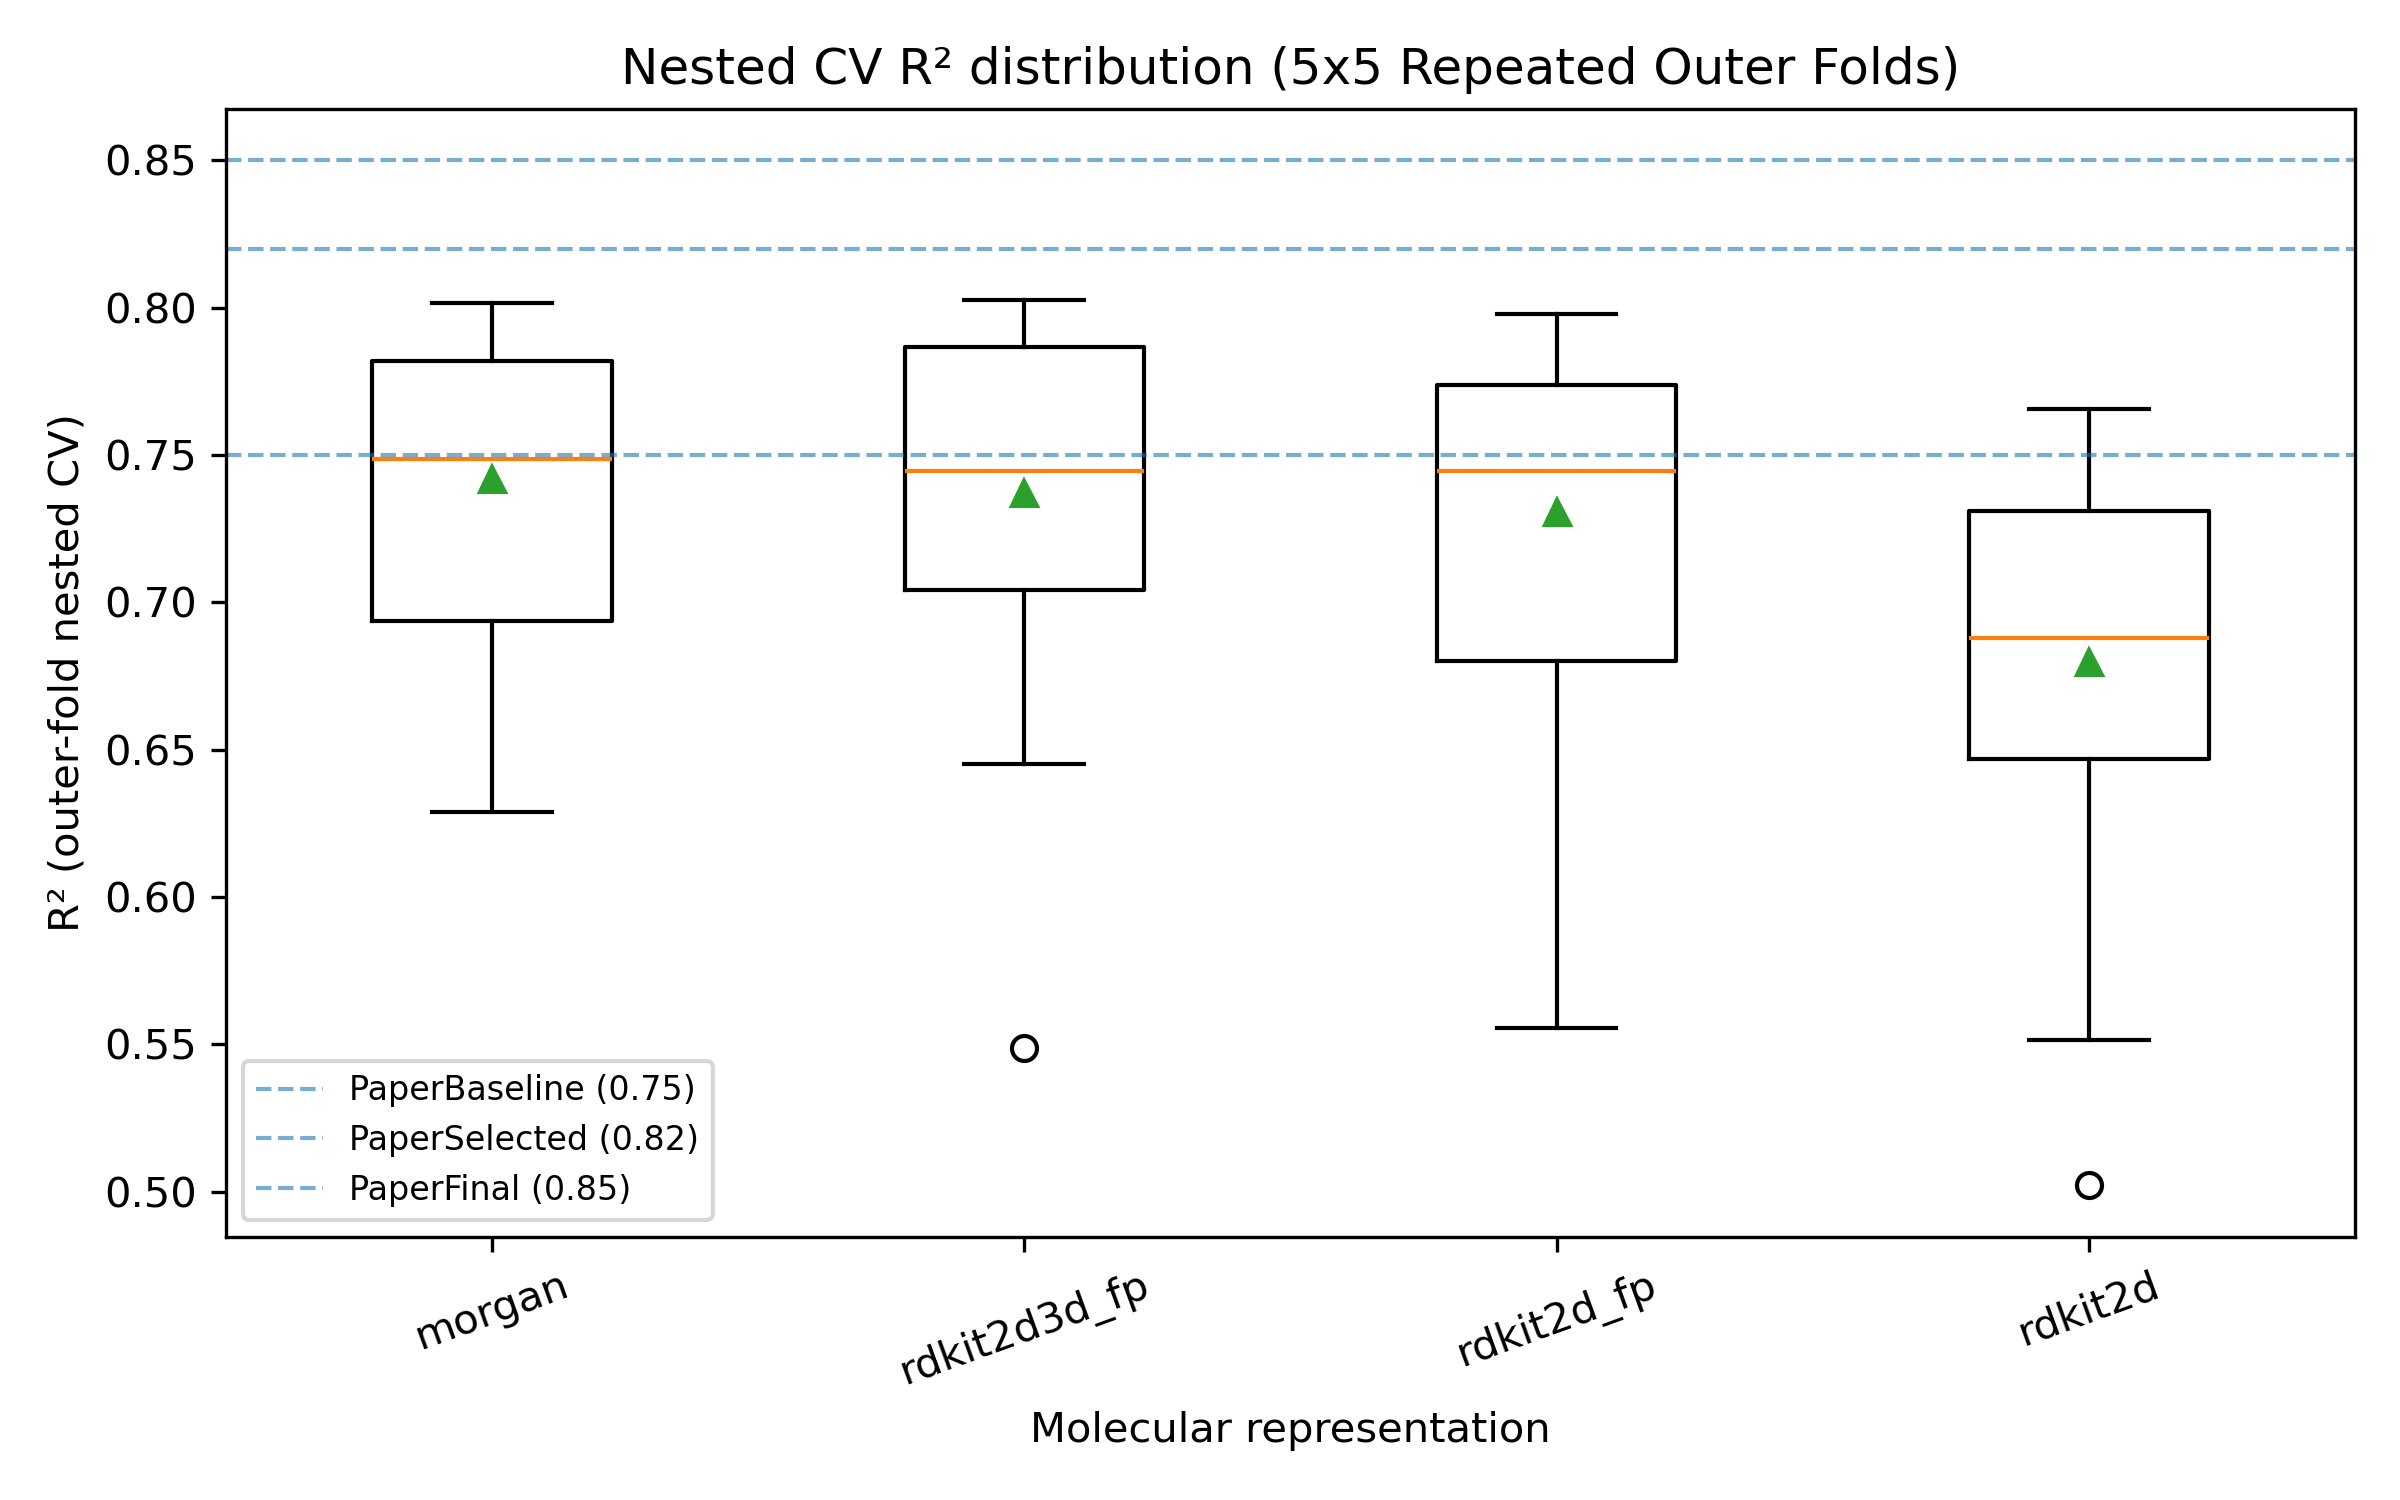
\includegraphics[width=0.8\textwidth]{figures/r2_by_representation_boxplot.png}
	\caption{Nested cross-validation $R^2$ distributions across four molecular representations. The purely structural Morgan fingerprint representation demonstrates equivalent predictive capacity to highly engineered 3D descriptors, establishing a robust classical baseline.}
	\label{fig:nested_cv_boxplot}
\end{figure}

Escalating feature complexity failed to yield commensurate predictive gains. Integrating RDKit 2D descriptors with Morgan fingerprints (analogous to the original study's ``2D/FP'' model) produced an $R^2$ of $\RdkitTwoDFpRTwoMean \pm \RdkitTwoDFpRTwoStd$ and an MAE of \RdkitTwoDFpMaeMean. The most complex representation, incorporating 3D geometric descriptors derived from ETKDGv3 embedding and MMFF94s optimization (analogous to the ``2D/3D/FP'' model), attained an $R^2$ of $\RdkitTwoDThreeDFpRTwoMean \pm \RdkitTwoDThreeDFpRTwoStd$ and an MAE of \RdkitTwoDThreeDFpMaeMean. A paired t-test comparing the purely structural Morgan fingerprint ensemble against the highly engineered 2D/3D/FP model revealed no statistically significant difference in explained variance ($t = \PairedTTestStat$, $p = \PairedTTestP$). To rigorously assess error magnitude differences while avoiding pseudoreplication artifacts, we applied a Nadeau-Bengio corrected paired t-test to the cross-validated MAE distributions. This confirmed the variance in absolute error lacks statistical significance ($t = \CorrectedTStat$, $p = \CorrectedTP$). These results indicate that conformational 3D featurization offers no measurable predictive advantage for this specific benchmark. Conversely, relying exclusively on 2D physicochemical descriptors severely degraded performance ($R^2 = \RdkitTwoDRTwoMean \pm \RdkitTwoDRTwoStd$, MAE = \RdkitTwoDMaeMean). Topological fingerprints act as the primary drivers of predictive capacity.

We benchmarked our highest-performing classical model against the incremental progression reported in the original study to contextualize the computational cost-benefit ratio of advanced statistical techniques (Table~\ref{tab:methodological_comparison}). Our classical stacking ensemble trained solely on Morgan features ($R^2 = \MorganRTwoMean$) performed comparably to their unselected 2D/3D/FP baseline model ($R^2 = \PaperBaselineRTwo$). Evaluated under a Nadeau-Bengio corrected one-sample $t$-test, this variance lacks statistical significance ($t = \TStatMorganVsPaperBaseline$, $p = \PValueMorganVsPaperBaseline$). Furthermore, our baseline 95\% bootstrap confidence interval $[\ExpARTwoCILow, \ExpARTwoCIHigh]$ strictly encompasses the literature baseline, confirming statistical parity. 

However, the literature model utilizing permutation importance-based feature selection ($R^2 = \PaperSelectedRTwo$) represents a statistically significant improvement over our unselected baseline ($t = \TStatMorganVsPaperSelected$, $p = \PValueMorganVsPaperSelected$), attributable to the supervised isolation of pharmacophoric signals. Similarly, the original study's final data-augmented deep neural network ensemble ($R^2 = \PaperFinalRTwo$) resides outside our baseline 95\% CI, representing a statistically significant deviation ($t = \TStatMorganVsPaperFinal$, $p = \PValueMorganVsPaperFinal$). These comparative results isolate the true source of predictive gains in this low-data regime. Achieving a competitive baseline performance ($R^2 \approx \PaperBaselineRTwo$) does not require computationally expensive 3D descriptors or complex neural network architectures; simple 2D fingerprints paired with classical machine learning algorithms suffice. The performance gaps between our baseline and the original study's advanced models directly quantify the impact of supervised feature selection and synthetic data augmentation rather than inherent architectural superiority.

\begin{table}[htbp]
	\centering
	\caption{Methodological comparison isolating the performance impact of architectural complexity, descriptor dimensionality, and data augmentation in TgDHFR bioactivity prediction.}
	\label{tab:methodological_comparison}
	\begin{tabular}{lllc}
		\toprule
		\textbf{Model Framework} & \textbf{Descriptors} & \textbf{Data Augmentation} & \textbf{Test $R^2$ (mean $\pm$ std)} \\
		\midrule
		Current Study (Classical Ensemble) & ECFP4 (2D) & None & \MorganRTwoMean $\pm$ \MorganRTwoStd \\
		Baseline \cite{karimova2025} & 2D/3D/FP & None & \PaperBaselineRTwo \textsuperscript{a} \\
		Augmented Final Model \cite{karimova2025} & 2D/3D/FP (Selected) & Gaussian Noise & \PaperFinalRTwo \textsuperscript{a} \\
		\bottomrule
		\multicolumn{4}{l}{\footnotesize \textsuperscript{a} Standard deviation not reported (NR) in the original study.}
	\end{tabular}
\end{table}
% ==========================================
% 3. SECTION 3.2
% ==========================================
\subsection{Benchmarking Tree-Based Ensembles Against Graph Neural Networks}

Graph Neural Networks (GNNs) dominate molecular property prediction by extracting representations directly from graph topologies. Their predictive utility, however, degrades sharply under data scarcity. To evaluate whether deep representation learning offers intrinsic advantages for the TgDHFR dataset (\NCompounds\ compounds), we benchmarked our optimal classical ensemble against a Directed Message Passing Neural Network (D-MPNN) using the Chemprop framework.

The D-MPNN yielded a cross-validated out-of-sample $R^2$ of $\ChemPropDMPNNFoldRTwoMean \pm \ChemPropDMPNNFoldRTwoStd$ and a Mean Absolute Error of \ChemPropDMPNNFoldMae. This network failed to match the classical stacking ensemble operating on pre-computed Morgan fingerprints ($R^2 = \MorganRTwoMean \pm \MorganRTwoStd$). This performance deficit stems directly from data scarcity and methodological asymmetry. The classical models underwent extensive hyperparameter optimization and architecture selection via the nested cross-validation pipeline. In contrast, the D-MPNN was evaluated using baseline hyperparameters without an equivalent exhaustive tuning phase. Restricted to \NCompounds\ training instances, the unoptimized D-MPNN cannot learn graph convolutions capable of surpassing the predictive baseline established by fixed, topological ECFP4 descriptors.

This convergence plateau provides contextual validation for the methodologies in the original study \cite{karimova2025}. The poor performance of the unaugmented D-MPNN explains the prior reliance on heavy statistical interventions—specifically, Gaussian data augmentation—to force predictive accuracy ($R^2 = \PaperFinalRTwo$, $p < 0.001$). Evaluated on unaugmented, data-limited chemical spaces, architectural complexity does not guarantee superior generalization. Classical tree-based ensembles utilizing fixed molecular descriptors remain the most robust, parsimonious, and computationally efficient alternative. Figure~\ref{fig:gnn_comparison} details the comparative performance across all baseline models and the GNN.

\begin{figure}[htbp] 
	\centering
	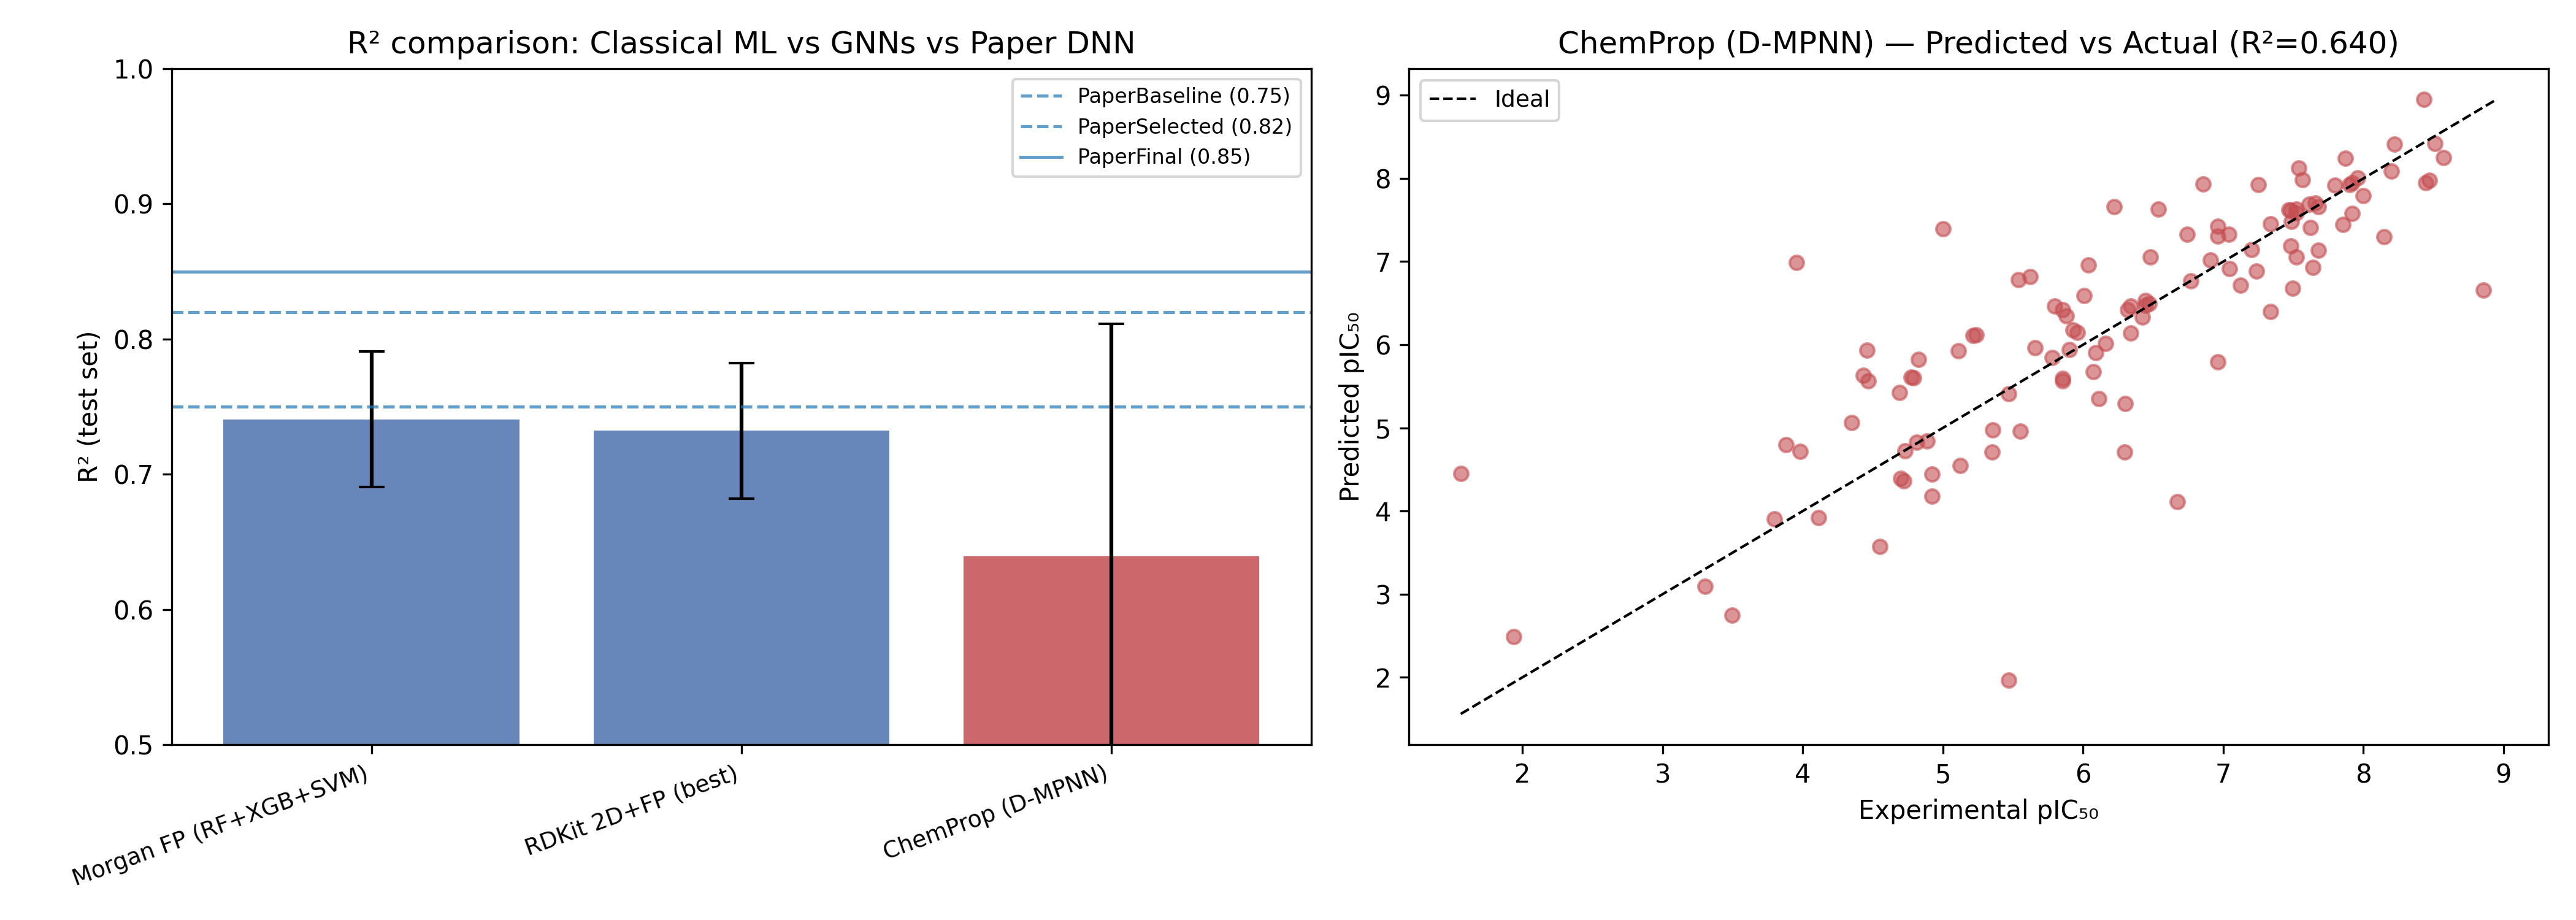
\includegraphics[scale=0.45]{figures/gnn_comparison.png} 
	\caption{Comparative predictive performance of classical machine learning ensembles, the Chemprop D-MPNN, and the original study's baseline and final models. The scatter plot details the predicted versus experimental $pIC_{50}$ values for the D-MPNN.}
	\label{fig:gnn_comparison} 
\end{figure}

% ==========================================
% 3. SECTION 3.3
% ==========================================
\subsection{Virtual Screening and Prioritization of FDA-Approved Candidates}

Transitioning from theoretical benchmarking to applied therapeutic discovery required deploying the optimized classical ensemble (\WinnerMode, $R^2 = \WinnerRTwoMean$) against a curated library of FDA-approved compounds. Prior to evaluating uncharacterized chemical spaces, the pipeline's predictive reliability underwent quantification using established TgDHFR inhibitors retained within the dataset. The algorithm recovered these internal controls with high fidelity. It assigned a predicted pIC$_{50}$ of 6.3259 to pyrimethamine (experimental: 6.56, absolute error: 0.2341) and 5.6352 to trimethoprim (experimental: 5.57, absolute error: 0.0652). This empirical alignment confirms the ensemble's capacity to interpolate bioactivity accurately within its defined applicability domain. To visualize this chemical space alignment, Principal Component Analysis (PCA) of the Morgan fingerprints confirmed that the prioritized FDA candidates fall strictly within the dense regions of the training distribution (Figure S1).

Following unsupervised Isolation Forest filtering to exclude structural outliers, the virtual screening protocol prioritized candidates based on absolute predicted potency and multi-objective ligand efficiency. Table~\ref{tab:fda_candidates} delineates the top ten prioritized compounds. Classic antifolate analogs—specifically methotrexate, trimetrexate, and folic acid—dominated the upper echelon of absolute affinity, all exceeding a predicted pIC$_{50}$ of 7.0. Absolute potency, however, frequently scales with molecular weight. This size dependency can artificially inflate binding scores and obscure the intrinsic thermodynamic quality of the underlying scaffold.

Correcting for physicochemical load via heavy-atom and molecular weight penalties revealed a distinct hierarchy of efficient binders. Smaller architectures demonstrated vastly superior atomic utilization. Pyrimethamine (LE = 0.51, BEI = 25.43), the potassium-sparing diuretic triamterene (LE = 0.48, BEI = 26.07), and the phenothiazine derivative methylene blue (LE = 0.45, BEI = 21.60) emerged as the most structurally optimized candidates. Triamterene and methylene blue provide particularly compelling repurposing profiles. They achieve robust predicted bioactivities while maintaining exceptional ligand efficiency indices, indicating highly complementary interactions with the TgDHFR catalytic pocket relative to their minimal steric footprints.

\begin{table}[htbp]
	\centering
	\caption{Top 10 FDA-approved candidates predicted by the classical ML model, ranked by predicted pIC$_{50}$ and evaluated across standard ligand efficiency metrics.}
	\label{tab:fda_candidates}
	\begin{tabular}{llccccc}
		\toprule
		\textbf{Rank} & \textbf{Compound Name} & \textbf{Predicted pIC$_{50}$} & \textbf{LE} & \textbf{BEI} & \textbf{LLE} & \textbf{SEI} \\
		\midrule
		1 & Methotrexate & 7.5678 & 0.31 & 16.65 & 7.30 & 3.59 \\
		2 & Trimetrexate Glucuronate (CID 54949) & 7.3351 & 0.25 & 13.02 & 7.88 & 2.90 \\
		3 & Trimetrexate Glucuronate (CID 336805) & 7.3351 & 0.25 & 13.02 & 7.88 & 2.90 \\
		4 & Folic Acid & 7.0830 & 0.30 & 16.05 & 7.13 & 3.32 \\
		5 & Methylene Blue & 6.9091 & 0.45 & 21.60 & 7.41 & 36.10 \\
		6 & Bendamustine Hydrochloride & 6.8859 & 0.39 & 17.44 & 3.20 & 11.39 \\
		7 & Fentanyl Citrate & 6.8673 & 0.25 & 12.99 & 3.98 & 4.41 \\
		8 & Ivabradine & 6.8497 & 0.28 & 14.62 & 3.54 & 11.33 \\
		9 & Ivabradine Hydrochloride & 6.8492 & 0.27 & 13.56 & 3.12 & 11.33 \\
		10 & Trifarotene & 6.8311 & 0.28 & 14.86 & 0.84 & 9.76 \\
		\bottomrule
	\end{tabular}
\end{table}
% ==========================================
% 3. SECTION 3.4
% ==========================================
\subsection{Integrated ML-docking consensus filtering and false-positive mitigation}

Standalone virtual screening methodologies generate false-positive artifacts. To mitigate this vulnerability, we implemented an orthogonal consensus filtering pipeline integrating ligand-based machine learning predictions with physics-based molecular docking. Spearman's rank correlation coefficient evaluated the global agreement between ML-predicted $pIC_{50}$ values and AutoDock Vina binding energies across the prioritized subset ($N = \DockNTotal$). This non-parametric approach ($\rho = \DockSpearmanRho$, $p = \DockSpearmanP$) handles restricted sample sizes and isolates monotonic trends without assuming linear dependencies between topological bioactivity interpolation and thermodynamic scoring.

The negative correlation confirms that higher predicted potencies trend with stronger binding energies. The absence of statistical significance ($p > 0.05$) validates the methodological design: two-dimensional ligand-based machine learning and three-dimensional physics-based docking capture fundamentally orthogonal aspects of molecular interaction. The ML ensemble interpolates bioactivity from topological patterns within the training distribution, whereas Vina calculates thermodynamic stability via spatial complementarity and electrostatic interactions. Relying on either method in isolation exposes the screening process to distinct classes of false positives.

The consensus approach identified and eliminated these methodological artifacts. Bisacodyl perfectly illustrates a physics-based false positive. It exhibited strong thermodynamic binding energies during structural validation ($\Delta G = -8.82\text{ kcal/mol}$), driven by the spurious accommodation of its flexible, hydrophobic scaffold within the binding pocket. The classical ML model, however, correctly assigned a low predicted affinity ($pIC_{50} = 5.25$) to this compound, vetoing its progression. Conversely, the ML model generated exactly \DockNDiscordant\ false positives; every candidate exceeding the ML potency threshold also satisfied the stringent docking energy criteria. Dual validation thus prevents the misallocation of experimental resources toward single-method screening artifacts.

Orthogonal docking isolated exactly \DockNValidated\ consensus hits from the \DockNTotal\ evaluated compounds that satisfied both the ML potency threshold ($pIC_{50} > 6.5$) and the stringent docking energy criteria ($\Delta G < -8.0\text{ kcal/mol}$). These validated hits are folic acid ($\Delta G = -8.62\text{ kcal/mol}$), methotrexate ($\Delta G = -8.68\text{ kcal/mol}$), pralatrexate ($\Delta G = -9.43\text{ kcal/mol}$), and triamterene ($\Delta G = -8.05\text{ kcal/mol}$). The primary consensus candidate, \DockBestCandidate, demonstrated a strong ML-predicted $pIC_{50}$ of \DockBestMLpIC\ alongside the most favorable docking score of \DockBestDockScore\ kcal/mol.

This lightweight, classical pipeline matches the statistical performance of unaugmented deep learning models while discovering biologically viable, physics-validated inhibitors. Isolating high-confidence repurposing candidates without synthetic data generation or 3D feature engineering yields a superior computational cost-benefit ratio for practical drug discovery in low-data regimes.
%\section{Discussion}

% ==========================================
% 4. SECTION 4.1 
% ==========================================

\subsection{The Role of Explicit Inductive Bias in Small-Scale Molecular Datasets}

Graph Neural Networks theoretically offer superior representational capacity by learning molecular features directly from graph topology, thereby bypassing the need for manual feature engineering. However, this architectural flexibility demands extensive training data to converge on generalizable chemical representations. In the context of the TgDHFR dataset, which comprises only \NCompounds\ compounds, the GNN architecture failed to leverage its theoretical superiority, plateauing at a predictive performance statistically indistinguishable from classical machine learning approaches. 

This convergence failure highlights the critical role of explicit inductive bias in low-data regimes. The fundamental lack of explicit chemical priors in deep representation learning forces these architectures to construct a continuous latent space entirely from scratch. With fewer than 1,000 training instances, the resulting latent space density is severely restricted, creating a sparse manifold where interpolation between data points becomes highly unstable. To counteract this sparsity, deep learning frameworks structurally require artificial variance injection. Consequently, achieving high predictive accuracy with neural networks on this specific dataset necessitates extensive Gaussian noise-based data augmentation, as demonstrated in the original study \cite{karimova2025}, to artificially inflate latent space density and force convergence.

Classical tree-based ensembles operating on pre-computed Morgan fingerprints bypass the need for end-to-end representation learning by utilizing fixed, domain-specific descriptors. These fingerprints encode established chemical heuristics—specifically, circular topological substructures—directly into the feature space. For small-scale datasets, this explicit pre-computation acts as a natural regularizer, rigidly constraining the hypothesis space and preventing the model from memorizing noise. Our results explicitly demonstrate that exploiting the inductive bias inherent to traditional structural fingerprints entirely eliminates the necessity for computationally burdensome data augmentation in this specific context. 

Nevertheless, this architectural superiority is strictly regime-dependent. While deterministic feature engineering provides a parsimonious and highly reliable strategy for the current low-data regime ($N = \NCompounds$), this advantage is expected to invert as the dataset scales. In high-data environments ($N \gg 1000$), the rigid constraints of pre-computed fingerprints typically become an informational bottleneck. Under those conditions, the flexible representational capacity of GNNs allows them to learn task-specific embeddings that systematically outperform classical descriptors.

% ==========================================
% 4. SECTION 4.2
% ==========================================

\subsection{Dimensionality, Conformational Overhead, and Model Efficiency}

Computational efficiency determines the practical viability of molecular representations in high-throughput virtual screening. Generating 3D geometric descriptors requires extensive conformational sampling and energy minimization (e.g., ETKDGv3 embedding and MMFF94s optimization). This conformational overhead scales non-linearly, creating severe processing bottlenecks when screening libraries expand into the millions of compounds.

Empirical results demonstrate that this computational expenditure provides no predictive advantage for TgDHFR inhibition. The composite 2D/3D/FP representation yielded an $R^2$ of \RdkitTwoDThreeDFpRTwoMean, which remains statistically indistinguishable from the purely topological Morgan fingerprint model ($R^2 = \MorganRTwoMean$; Nadeau-Bengio corrected $p = \CorrectedTP$). This parity confirms that 2D connectivity matrices capture the requisite pharmacophoric variance.

Parsimony therefore drives the optimal screening strategy. Excluding 3D descriptors and synthetic data augmentation eliminates processing latency during both feature extraction and model training. For this specific target, high-dimensional representations introduce computational friction without improving model fidelity. Consequently, lightweight 2D fingerprint ensembles offer a strictly superior, highly scalable architecture for virtual screening under constrained data conditions.

% ==========================================
% 4. SECTION 4.3
% ==========================================

\subsection{Methodological Scope, Limitations, and Translational Potential}

The predictive reliability of any quantitative structure-activity relationship (QSAR) model is inherently bounded by the chemical diversity of its training corpus. Given the dataset size of \NCompounds\ compounds, the applicability domain of our optimized ensemble is strictly restricted to the structural scaffolds and physicochemical properties represented within the curated TgDHFR data. Consequently, extrapolating predictions to highly divergent chemotypes or novel synthetic spaces carries an increased risk of reduced predictive confidence. 

A specific vulnerability intrinsic to 2D circular fingerprints in low-data regimes is their susceptibility to activity cliffs—pairs of structurally similar molecules that exhibit radically divergent bioactivities due to subtle chemical modifications. A single bioisosteric substitution or methylation can alter a critical hydrogen bond or steric fit within the binding pocket. Because Morgan fingerprints map topological neighborhoods into bit vectors without explicitly encoding 3D spatial conformation or electrostatic field potentials, they risk mapping active and inactive cliff-forming analogs to virtually identical representations. We strategically mitigated this limitation through our downstream multi-tier architecture. The orthogonal integration of physics-based molecular docking explicitly evaluates 3D spatial complementarity and steric clashes, acting as a structural filter that detects activity cliffs otherwise invisible to pure 2D topological models.

An additional methodological constraint involves the extensive architecture search executed within the inner optimization loop. Evaluating up to 41 distinct stacking combinations across six regressor families introduces a latent risk of model selection bias. While the nested cross-validation framework mathematically isolates this optimization phase from the outer test folds—thereby mitigating spurious performance inflation—it does not entirely eliminate architectural instability. To transparently quantify this variance, Supplementary Table S1 details the selection frequency of each meta-ensemble across the \TotalOuterFolds\ outer folds. Within the optimal Morgan fingerprint space, the \MorganBestArchitecture\ configuration emerged as the most stable architecture, yet it was selected in only \MorganStability\% of the iterations. This distribution confirms that while the nested design successfully prevents test-set leakage, the inherent data sparsity of the \NCompounds-compound benchmark inevitably restricts the convergence of the inner loop onto a single, universally dominant stacking hierarchy.

Despite these boundary conditions, the programmatic pipeline developed in this study exhibits high transferability to other neglected tropical diseases (NTDs) and orphan targets. Because the framework relies on classical ensemble learning rather than data-hungry deep neural networks, it maintains predictive stability in low-data regimes (e.g., datasets with fewer than 1,000 compounds). This architecture provides a computationally lightweight triage mechanism that can be rapidly deployed for other under-researched pathogens. By systematically filtering extensive libraries of approved drugs to isolate a tractable subset of candidates, the pipeline minimizes the computational overhead required for subsequent physics-based simulations and reduces the attrition rate in downstream experimental validations.

Finally, the integration of ADMET profiling contextualizes the clinical viability of the prioritized candidates. The top-ranked hybrid hit, Pralatrexate (\DockBestDockScore\ kcal/mol), alongside the reference drug Methotrexate, exhibited low predicted Caco-2 permeability, classifying them as parenteral rather than oral candidates. Rather than a limitation, this pharmacokinetic profile is mechanistically consistent with classical antifolates, which are typically highly polar, structurally complex molecules. Clinically, parenteral administration aligns directly with the treatment protocols for severe, acute manifestations of the disease, such as toxoplasmic encephalitis in immunocompromised patients, where intravenous delivery ensures rapid systemic bioavailability. Consequently, the pipeline not only identifies potent target binders but also accurately anticipates their clinical administration routes, reinforcing its utility in applied pharmacological repurposing.


%\subsection{Conclusions and Future Directions}

This study re-evaluates the methodological prerequisites for molecular property prediction in low-data environments ($N = \NCompounds$), yielding three principal findings. First, classical machine learning ensembles operating on 2D topological fingerprints provide sufficient explicit inductive bias ($R^2 = \MorganRTwoMean \pm \MorganRTwoStd$) to surpass the predictive utility of unaugmented deep learning architectures ($R^2 = \ChemPropDMPNNFoldRTwoMean$) and computationally expensive 3D descriptors. This advantage, however, remains strictly bounded to low-data regimes where complex neural architectures suffer from parameter underdetermination. Second, rigorous nested cross-validation remains imperative to eliminate optimistic performance bias and accurately quantify out-of-sample generalization. 

Third, integrating ligand-based statistical predictions with physics-based molecular docking and ADMET profiling establishes a robust consensus filter. This orthogonal validation mitigates the false-positive rates inherent to isolated screening methodologies. By enforcing strict pharmacokinetic constraints—specifically evaluating hERG cardiotoxicity and Caco-2 intestinal permeability—the pipeline isolates \DockNValidated{} structurally and translationally viable candidates. Most notably, \DockBestCandidate{} emerges as a high-priority candidate for therapeutic repurposing, demonstrating both strong predicted affinity and a compliant safety profile. 

Future investigations must transition these computational findings into experimental validation. \textit{In vitro} enzymatic assays are required to confirm the inhibitory kinetics of \DockBestCandidate{} and the remaining consensus candidates against TgDHFR. Subsequent \textit{in vivo} efficacy models in \textit{Toxoplasma gondii}-infected cohorts will determine their systemic viability. Additionally, expanding the computational framework to evaluate multi-target selectivity profiles—specifically quantifying the binding affinity differential between TgDHFR and human DHFR—will be necessary to anticipate and minimize off-target toxicity in clinical applications.

\section*{Data and Code Availability}

All source code, Python scripts for dataset processing, nested cross-validation, model training, and docking validation protocols, as well as the benchmark datasets, are publicly available in the GitHub repository at the following \href{https://github.com/aavzpy2023/analysispaperKarimova2025}{\underline{link}}

\section*{Declaration of Generative AI's use}

During the preparation of this work, the author(s) utilized generative artificial intelligence technologies (Large Language Models) solely to assist with language polishing, structural formatting, and improving the overall readability of the manuscript. After using these tools, the author(s) thoroughly reviewed, edited, and validated all generated text. The author(s) take full and sole responsibility for the final content, scientific integrity, and accuracy of this publication. No AI technologies were used to generate data, perform statistical analyses, or draw scientific conclusions.

\bibliographystyle{ieeetr}
\bibliography{references}


\end{document}